\documentclass{article}
\usepackage{amsfonts, amsmath, amssymb, amsthm} % Math notations imported
\usepackage{enumitem}
\usepackage{graphicx}
\usepackage{setspace}
\usepackage{indentfirst}
\usepackage[margin=1in]{geometry}
\graphicspath{{./images/}} % Path to images

% \begin{figure}[htb!]
%      \centering
%      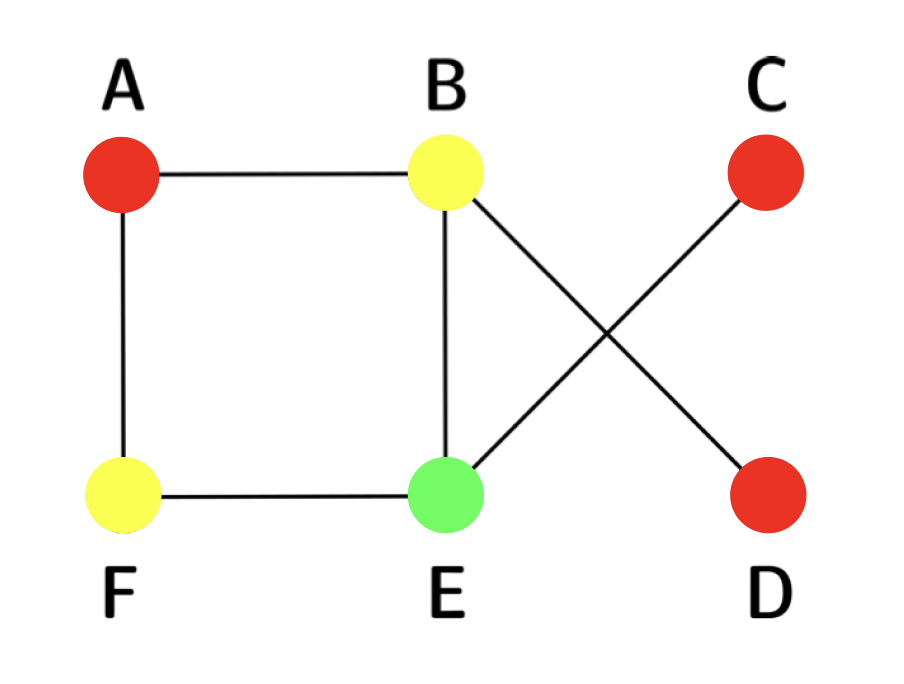
\includegraphics[scale=0.5]{coloring.png}
%      \caption{Coloring of the graph.}
% \end{figure}

% \begin{figure}[htb]
%     \qquad
%     \begin{minipage}{.4\textwidth}
%         \centering
%         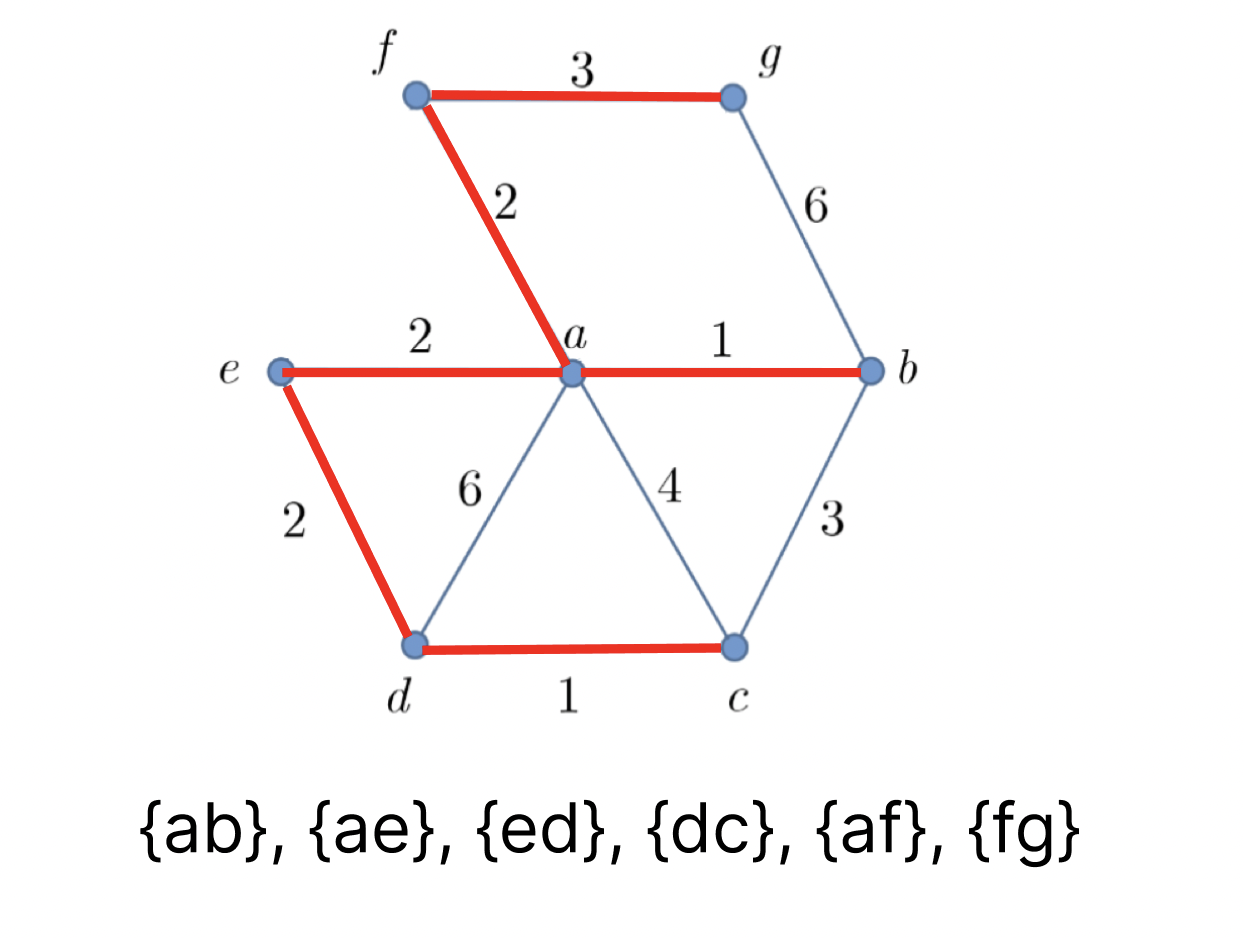
\includegraphics[scale=0.35]{prims.png}
%         \caption{}
%     \end{minipage}    
%     \qquad
%     \begin{minipage}{.4\textwidth}
%         \centering
%         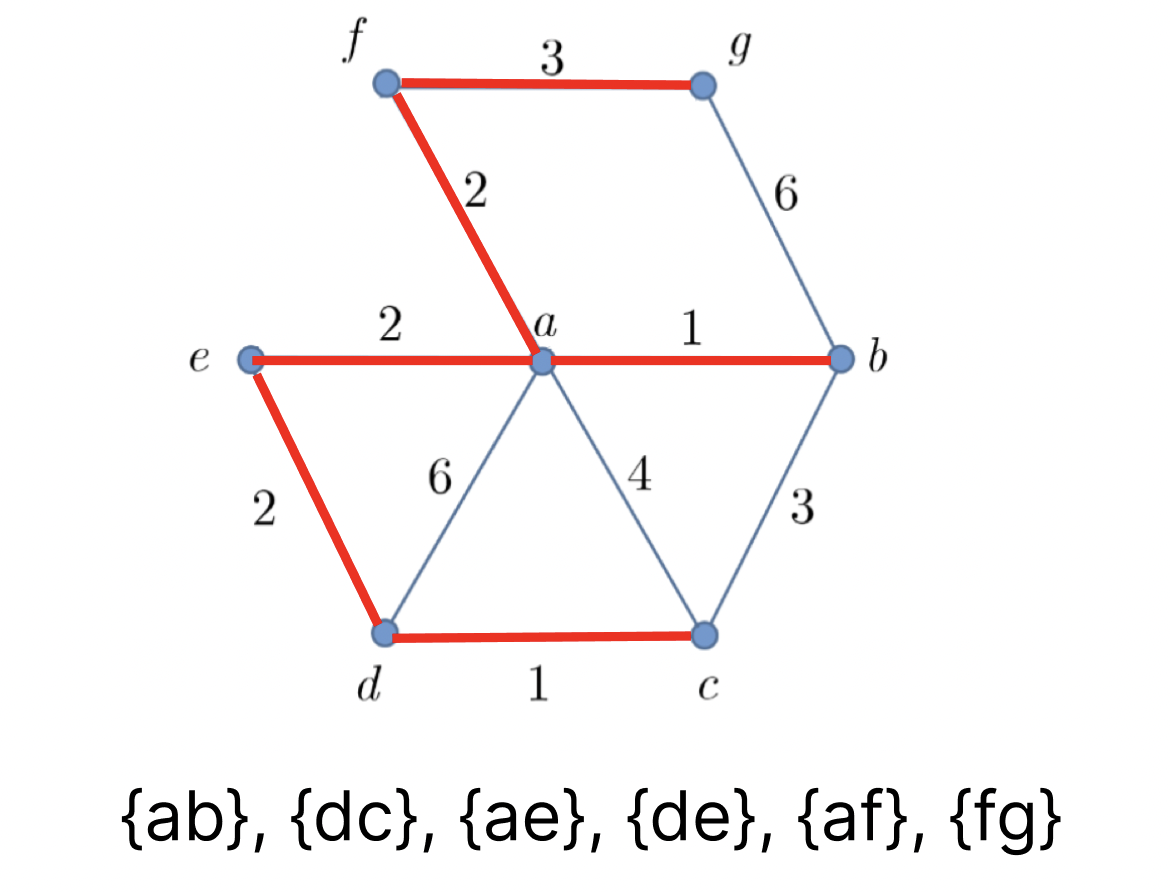
\includegraphics[scale=0.35]{kruskal.png}
%         \caption{}
%     \end{minipage}        
% \end{figure} 

\newtheorem{thm}{Theorem}
\newtheorem{proposition}[thm]{Proposition}
\newtheorem{cor}[thm]{Corollary}

% title information
\title{Math 110 HW6}
\author{Neo Lee}
\date{10/07/2023}

\setstretch{1.15}
% main content
\begin{document} 

% placing title information; comment out if using fancyhdr
\maketitle 

\section*{Problem 1.}
Suppose $q\in {\cal P}(\mathbb{R})$. Prove that there exists a polynomial 
$p\in {\cal P}(\mathbb{R})$ such that
$$ q(x)= (x^2-3x)p''(x) +(2x-3) p'(x)+p(0).$$
\begin{proof}
    We want to show that this map, specifically a linear map, is surjective. Denote the map as $T$. 

    We first show that this is a linear map.
    Consider $p_1$ and $p_2$, then 
    \begin{align*}
        T(p_1+p_2)(x) & = (x^2-3x)(p_1+p_2)''(x) +(2x-3) (p_1+p_2)'(x)+(p_1+p_2)(0) \\
        & = (x^2-3x)(p_1''+p_2'')(x) +(2x-3) (p_1'+p_2')(x)+(p_1+p_2)(0) \\
        & = (x^2-3x)p_1''(x) +(2x-3) p_1'(x)+p_1(0) + (x^2-3x)p_2''(x) +(2x-3) p_2'(x)+p_2(0) \\
        & = T(p_1)(x) + T(p_2)(x).
    \end{align*}
    Consider $\lambda \in \mathbb{F}$, then 
    \begin{align*}
        T(\lambda p)(x) & = (x^2-3x)(\lambda p)''(x) +(2x-3) (\lambda p)'(x)+(\lambda p)(0) \\
        & = \lambda(x^2-3x)p''(x) +\lambda(2x-3) p'(x)+\lambda p(0) \\
        & = \lambda \left((x^2-3x)p''(x) +(2x-3) p'(x)+p(0)\right) \\
        & = \lambda T(p)(x).
    \end{align*}

    Next for each $q\in\mathcal{P}(\mathbb{R})$, we restrict the domain and codomain of $T$ to 
    $\mathcal{P}_m(\mathbb{R})$ for $m=$ degree$(q)$. Then we show that for each 
    $q\in\mathcal{P}(\mathbb{R})$, $T:\mathcal{P}_m(\mathbb{R})\to\mathcal{P}_m(\mathbb{R})$ is 
    injective, hence surjective. Consider 
    \begin{align*}
        T(p) & = \vec{0} \\
        (x^2-3x)p''(x) +(2x-3) p'(x)+p(0) & = \vec{0}.
    \end{align*}
    Notice if $p$ is of degree $\ge 1$, the left hand side is a degree $\ge 1$ 
    polynomial and cannot be the zero map. If $p$ is of degree 0, which is a non-zero constant, then 
    left hand side is a constant function, which again cannot be the zero map. Hence, in conclusion 
    the only possible $p$ is the zero polynomial function. Therefore, null $T = \{0\}$, and $T$ is 
    injective. Since we restricted the map $T:\mathcal{P}_m(\mathbb{R})\to
    \mathcal{P}_m(\mathbb{R})$ for each $q$, the domain and codomain of 
    $T$ have the same finite dimension and injectivity implies surjectivity.
\end{proof}

\newpage
\section*{Problem 2.}
Let $V$ be a vector space over $\mathbb{F}$. Give a constructive proof that $V$ and 
${\cal L}(\mathbb{F}, V)$ are isomorphic, i.e., construct an explicit isomorphism between 
these spaces.
\begin{proof}[Solution]
    Define $T_v: x\to xv$, for $x\in\mathbb{F}, v\in V$. 
    \begin{align*}
        T_v(x_1+x_2) & = (x_1+x_2)v \\
        & = x_1v + x_2v \\
        & = T_v(x_1) + T_v(x_2). \\
        T_v(\lambda x) & = (\lambda x)v \\
        & = \lambda (xv) \\
        & = \lambda T_v(x).
    \end{align*}
    Therefore, $T_v$ is a linear map and is indeed in $\mathcal{L}(\mathbb{F}, V)$.

    Now define $\Phi:v\to T_v$. 
    \begin{align*}
        \Phi(v_1+v_2)(x) & = T_{v_1+v_2}(x) \\
        & = x(v_1+v_2) \\
        & = xv_1 + xv_2 \\
        & = T_{v_1}(x) + T_{v_2}(x) \\
        & = \Phi(v_1)(x) + \Phi(v_2)(x). \\
        \Phi(\lambda v)(x) & = T_{\lambda v}(x) \\
        & = x(\lambda v) \\
        & = \lambda (xv) \\
        & = \lambda T_v(x) \\
        & = \lambda \Phi(v)(x).
    \end{align*}
    Therefore, $\Phi$ is indeed a linear map.

    Now we show that $\Phi$ is injective. Consider the zero map in $\mathcal{L}(\mathbb{F}, V)$, 
    in order for $\Phi$ to map to the zero map, we need $T_v(x) = xv = 0$ for all $x\in\mathbb{F}$, which is 
    only possible when $v=0$. Hence, null $\Phi = \{0\}$, and $\Phi$ is injective.
    
    Now we show that $\Phi$ is surjective. Notice $$\dim \mathrm{range }T = \dim V - \dim \mathrm{null }T = \dim V
    = \dim \mathbb{F}\times \dim V = \dim \mathcal{L}(\mathbb{F}, V),$$
    thus $\mathrm{range }T = \mathcal{L}(\mathbb{F}, V)$. Hence, $\Phi$ is surjective.

    Therefore, $\Phi$ is an isomorphism between $V$ and $\mathcal{L}(\mathbb{F}, V)$.
\end{proof}

\newpage
\section*{Problem 3.}
Which of the following maps on ${\cal P}(\mathbb{R})$ are linear functionals?\smallskip
 
 (a) $p(x)\mapsto \int_{-1}^{x} p(t) dt$\smallskip
 
 (b) $p(x)\mapsto \int_{0}^1 p(4t^{10}+t^3-1) dt$\smallskip
 
 (c) $p(x)\mapsto p(0)p''(\pi)$\smallskip
 
 (d) $p(x) \mapsto 2p(1)$
\begin{proof}[Solution]\indent
    \begin{enumerate}[label=(\alph*)]
        \item This is not a linear functionals. Let $P(x)\in\mathcal{P}(\mathbb{R})$ such that $\frac{dP}{dx}
        = p$. Then $$\int_{-1}^{x}p(t) = P(x)-P(1),$$ which is a polynomial function instead of a 
        field. 

        \item
        This is a linear functional. Indeed a definite integral will evaluate to a constant, which is 
        a field. Consider $p_1, p_2\in\mathcal{P}(\mathbb{R})$, then
        \begin{align*}
            T(p_1+p_2) & = \int_{0}^1 (p_1+p_2)(4t^{10}+t^3-1) dt \\
            & = \int_{0}^1 p_1(4t^{10}+t^3-1) dt + \int_{0}^1 p_2(4t^{10}+t^3-1) dt \\
            & = T(p_1) + T(p_2).
        \end{align*}
        Consider $\lambda\in\mathbb{F}$, then
        \begin{align*}
            T(\lambda p) & = \int_{0}^1 (\lambda p)(4t^{10}+t^3-1) dt \\
            & = \lambda \int_{0}^1 p(4t^{10}+t^3-1) dt \\
            & = \lambda T(p).
        \end{align*}
        Hence, it is linear.

        \item
        This is not a linear functional. Consider $p_1, p_2\in\mathcal{P}(\mathbb{R})$ such that
        $p_1(x)=1$ and $p_2(x)=x^2$, then
        \begin{align*}
            T(p_1+p_2) & = (p_1+p_2)(0)(p_1+p_2)''(\pi) \\
            & = \left(p_1(0)+p_2(0)\right)(p_1''(\pi)+p_2''(\pi)) \\
            & = (1+0)(0+2) \\
            & = 2 \\
            & \neq 0 + 0 = p_1(0)p''(\pi) + p_2(0)p_2''(\pi).
        \end{align*}

        \newpage
        \item
        This is a linear functional. Indeed an evaluation of a polynomial function at a point will 
        evaluate to a constant, which is a field. Consider $p_1, p_2\in\mathcal{P}(\mathbb{R})$, 
        then
        \begin{align*}
            T(p_1+p_2) & = 2(p_1+p_2)(1) \\
            & = 2p_1(1) + 2p_2(1) \\
            & = T(p_1) + T(p_2).
        \end{align*}
        Consider $\lambda\in\mathbb{F}$, then
        \begin{align*}
            T(\lambda p) & = 2(\lambda p)(1) \\
            & = \lambda (2p(1)) \\
            & = \lambda T(p).
        \end{align*}
        Hence, it is linear.
    \end{enumerate}
\end{proof}

\newpage
\section*{Problem 4.}
Let $V={\cal P}_2(\mathbb{R})$ and suppose $\varphi_j(p)=p(j-1)$, $j=1,2,3$.
Prove that $(\varphi_1, \varphi_2, \varphi_3)$ is a basis for ${\cal P}_2(\mathbb{R})'$ and find a 
basis $(p_1,p_2,p_3)$ of ${\cal P}_2(\mathbb{R})$ whose dual is $(\varphi_1, \varphi_2, \varphi_3)$.
\begin{proof}
    $(\varphi_1, \varphi_2, \varphi_3)$ is of length 3 while $\dim{\cal P}_2(\mathbb{R})'=3$, thus 
    it suffices to show that $(\varphi_1, \varphi_2, \varphi_3)$ is linearly 
    independent.

    Consider $\alpha, \beta, \gamma\in\mathbb{R}$ and $p = ax^2+bx+c\in\mathcal{P}(\mathbb{R})$, then 
    \begin{align*}
        \alpha\varphi_1(p) + \beta\varphi_2(p) + \gamma\varphi_3(p) & = 0 \\
        \alpha p(0) + \beta p(1) + \gamma p(2) & = 0 \\
        \alpha c + \beta(a+b+c) + \gamma(4a+2b+c) & = 0 \\
        a(4\gamma+\beta) + b(2\gamma+\beta) + c(\alpha+\beta+\gamma) & = 0.
    \end{align*}
    Since $a, b, c$ are arbitrary, we must have
    \begin{align*}
        \begin{cases}
            4\gamma+\beta = 0 \\
            2\gamma+\beta = 0 \\
            \alpha+\beta+\gamma = 0
        \end{cases}
        \implies 
        \begin{cases}
            \gamma = 0 \\
            \beta = 0 \\
            \alpha = 0
        \end{cases}.
    \end{align*}
    Hence, $(\varphi_1, \varphi_2, \varphi_3)$ is linearly independent and is a basis for
    ${\cal P}_2(\mathbb{R})'$.

    To find the corresponding basis $(p_1, p_2, p_3)$, we need 
    \begin{align*}
        \begin{cases}
            p_1(0) = 1, p_1(1) = 0, p_1(2) = 0 \\
            p_2(0) = 0, p_2(1) = 1, p_2(2) = 0 \\
            p_3(0) = 0, p_3(1) = 0, p_3(2) = 1
        \end{cases}
    \end{align*}
    Define $p_1(x) = \frac{(x-1)(x-2)}{2}$, $p_2(x) = -x(x-2)$, and $p_3(x) = \frac{x(x-1)}{2}$. 
    Indeed, these 3 functions satisfy the above conditions, so it suffices to show that 
    they are linear independent. Consider $\alpha, \beta, \gamma\in\mathbb{R}$, then
    \begin{align*}
        \alpha p_1(x) + \beta p_2(x) + \gamma p_3(x) & = 0 \\
        \alpha \frac{(x-1)(x-2)}{2} + \beta (-x(x-2)) + \gamma \frac{x(x-1)}{2} & = 0 \\
        \alpha (x^2-3x+2) - 2\beta (x^2-2x) + \gamma (x^2-x) & = 0 \\
        (\alpha-2\beta+\gamma)x^2 + (-3\alpha+4\beta-\gamma)x + (2\alpha) & = 0.
    \end{align*}
    We already know that $x^2, x, 1$ are linearly independent, thus we must have
    \begin{align*}
        \begin{cases}
            \alpha-2\beta+\gamma = 0 \\
            -3\alpha+4\beta-\gamma = 0 \\
            2\alpha = 0
        \end{cases}
        \implies 
        \begin{cases}
            \alpha = 0 \\
            \beta = 0 \\
            \gamma = 0
        \end{cases}.
    \end{align*}
    Therefore, $(p_1, p_2, p_3)$ is linearly independent and is a basis for ${\cal P}_2(\mathbb{R})$.
\end{proof}

\newpage
\section*{Problem 5.}
Let $V$ be a finite-dimensional vector space and let $U$ be its proper subspace 
(i.e., $U\neq V$). Prove that there exists $\varphi\in V'$ such that $\varphi(u)=0$ for all $u\in U$ 
but $\varphi\neq 0$.
\begin{proof}
    It's equivalent to showing that the annihilator of $U$ contains non-trivial vector. Since $U$ is 
    a subspace of $V$, we have 
    $$\dim U^0 = \dim V - \dim U > 0 \qquad \because \dim U < \dim V.$$
    Therefore, the annihilator of $U$ contains non-trivial vector.
\end{proof}
\end{document}
